\section{Case studies}

\subsection{Jones Polynomial at Lattice Roots of Unity}

For $d=2,3,4$ it's easy.
For $d\geq 5$ it's hard.

Mention Potts and also anyon stuff but the important thing is the tensornet.

A knot $K$ is a circle embedded in $\mathbb{R}^3$.
A set of knots tangled together is a \emph{link} $L$.
A link $L$ is represented as the projection of the link on $\mathbb{R}^2$
but retaining the information of over or under crossings.
For example, the trefoil knot linked with an unknot can be drawn as:

\begin{equation}
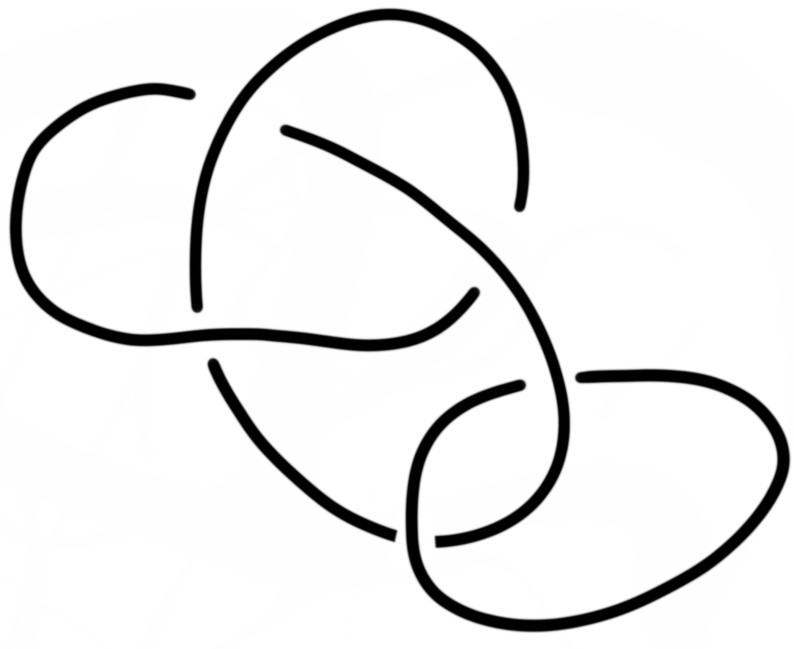
\includegraphics[scale=0.2]{figures/link.jpg}
\label{eq:link}
\end{equation}

We say that $L\simeq L'$ if there is a sequence of Reidemeister moves from $L$ to $L'$, i.e. reversible local strand deformations that do not change the topology, for example by cutting or gluing strands (see Appendix).

The Jones polynomial $V_L(t)$
is a Laurent polynomial in $t\in\mathbb{C}$
and is a link \emph{invariant}.
This means that
$V_L(t)\neq V_{L'}(t)\Rightarrow L\not\simeq L'$,
where $L\simeq L'$.

In general, computing $V_L(t)$
is exponentially costly in the number of crossings $|C|$,
something made explicit when one uses the Kauffman bracket method where a skein relation is used iteratively on every crossing [KauffmanBook].
Exactly evaluating the Jones polynomial at specific points $t\in\mathbb{C}$ is \#P-hard.
\emph{except} at the \emph{lattice roots of unity} $\pm 1, \pm i, \pm e^{i 2\pi/3}, \pm e^{i 4\pi/3}$ where it can be evaluated efficiently (in time $O(poly(|C|))$) [Welsh].


In the context of quantum computation,
additively approximating the Jones polynomial at non-lattice roots of unity is the paradigmatic BQP-complete complete problem [aharonov].
For the lattice roots of unity, the quantum amplitude to which the problem reduces can be computed efficiently.
Specifically, the quantum circuits that need to be simulated are stabiliser circuits which are known to be classically tractable [ref? Kuperberg? Aharonov?].
From the more natural point of view of topological quantum computation,
the jones polynomial at roots of unity corresponds to a quantum amplitude in the fusion space of non-abelian anyons.
Computation is performed by initialising, braiding, and the anyons.
Specifically, in the case of $\text{SU}(2)_k$ anyons, the Jones polynomial is evaluated at $e^{i\frac{2\pi}{2+k}}$ [Rowel-Wang]. Note the correspondence $q\in\{1,2,3,4\}\Leftrightarrow k\in{1,2,4}$.
This is consistent with the fact that topological quantum computation with $\text{SU}(2)_2$ anyons (Ising) or $\text{SU}(2)_4$ anyons is not universal (unless the $\text{SU}(2)_4$ anyons are augmented by fusion and measurements in which case they are capable of universal quantum computation [1504.02098]).



Remarkably, the Jones polynomial can be expressed in terms of the partition function of a $q$-state Potts model [Wu].
The Potts model is defined on a signed graph, called the Tait graph, which is obtained as follows.
The link diagram is bicoloured (checkerboard style)
and every coloured area is mapped to a vertex and every crossing is mapped to a signed edge according
its orientation relative to the surrounding colours.
Every vertex is assigned a $q$-state classical spin
and every signed edge indicates a spin-spin Tait-sign-dependent interaction $J_\pm\in\mathbb{C}$ which relate to the Jones polynomial's variable as $e^{J_\pm}=-t^\mp$.
The role of the link invariant is played by the partition function $Z(q)$;
in fact, the interactions $J_\pm$ are such so that the graph operations corresponding to Reidemeister moves leave $Z(q)$ invariant.
Multiplying with an efficiently computatble prefactor $\mathcal{A}(t) = (-t^\frac{1}{2}-t^{-\frac{1}{2}})^{(-|V|-1)} (-t^\frac{3}{4})^w t^{\frac{1}{4}\tau}$ for bookkeeping of twist factors, the relation to the Jones polynomial is
$V_L(t) = \mathcal{A}(t) Z(q)$.
The link shown in Eq.\ref{eq:link} returns the following tensor network.


\begin{equation}
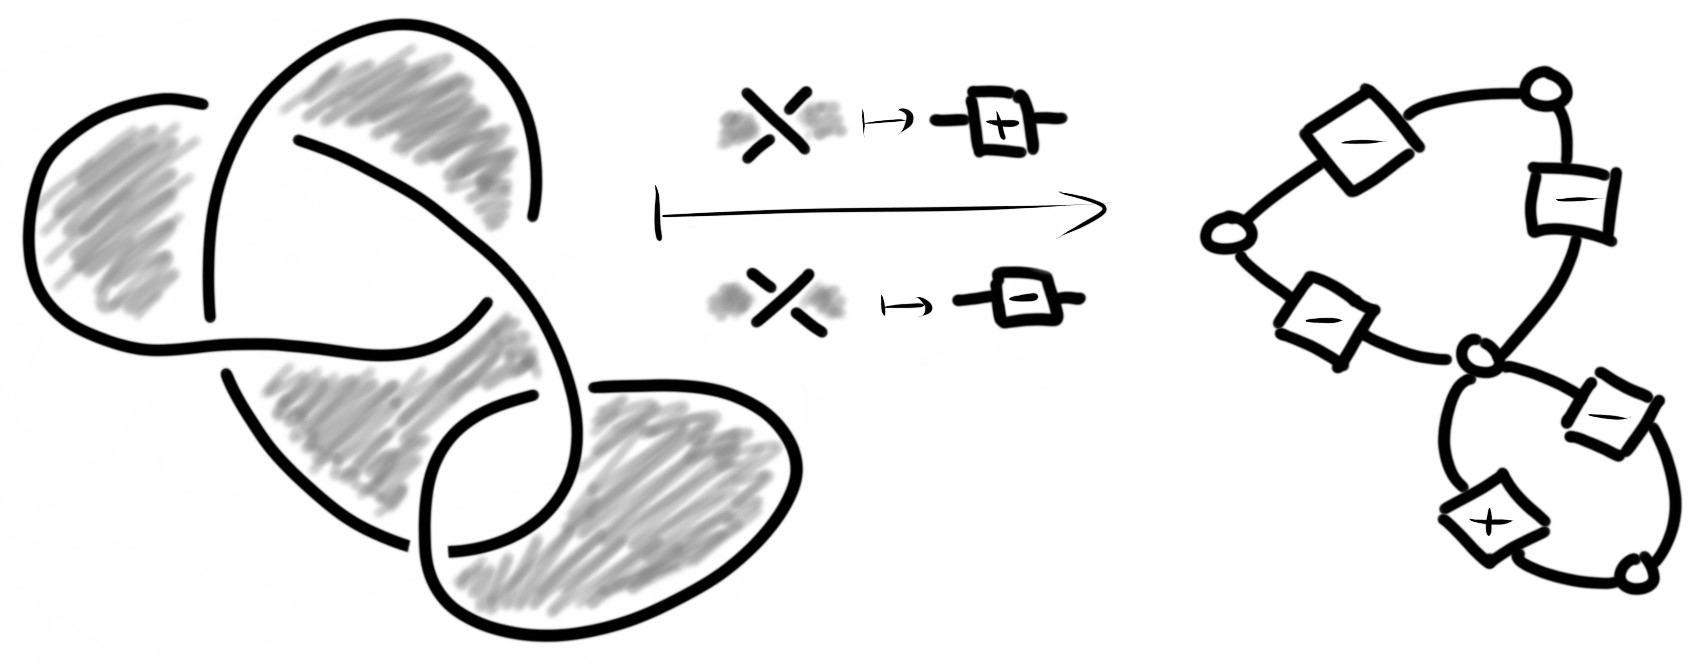
\includegraphics[scale=0.2]{figures/link-tn.jpg}
\label{eq:link-tn}
\end{equation}



For $q=2$ in ZX notation:
\begin{equation}
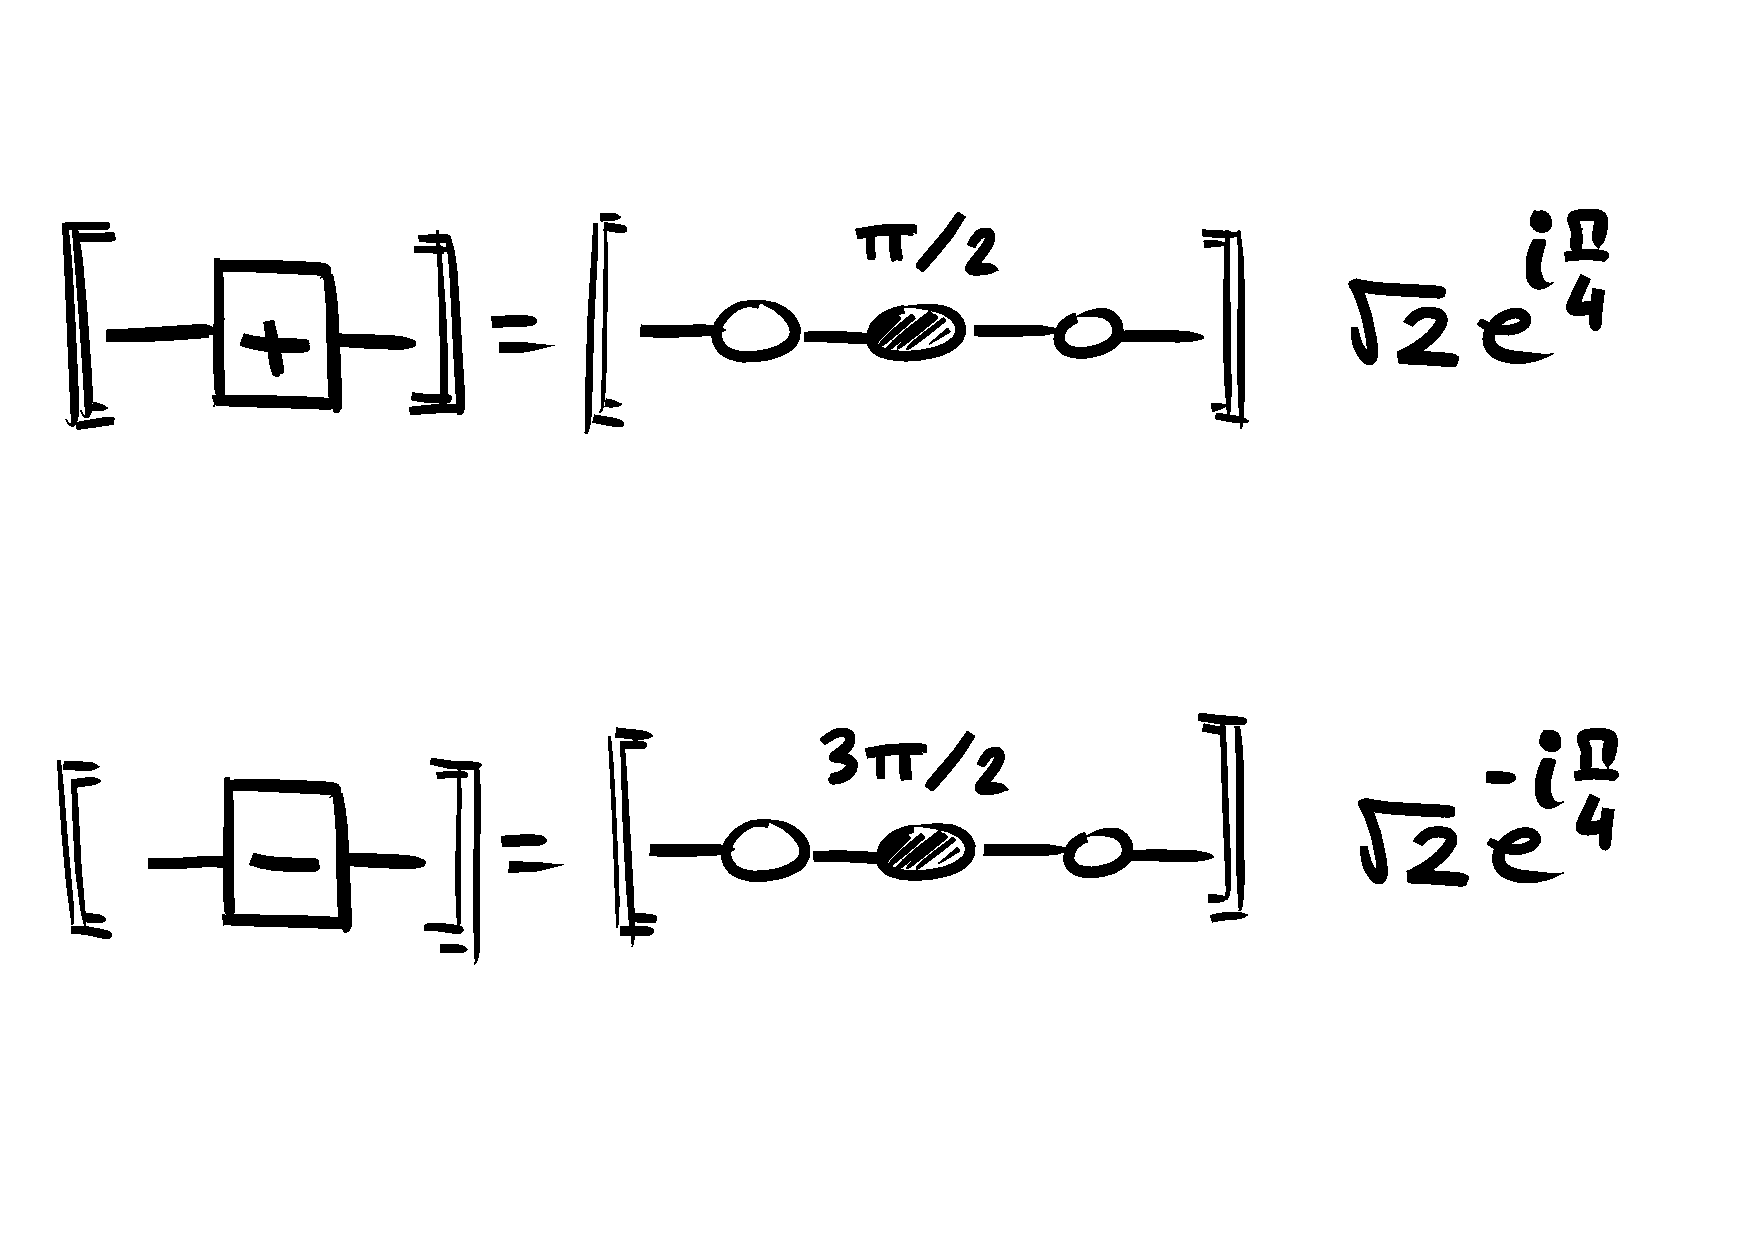
\includegraphics[scale=0.15]{figures/q2.pdf}
\end{equation}





We provide a graphical proof that
evaluating the Jones polynomial of arbitrary links at the lattice roots of unity is in P. For these cases, the problem reduces to the evaluation of the partition function of a planar $q$-state Potts model.
The partition is represented as a closed tensor network.
We employ the ZX-calculus,
which is a sound and complete graphical language
for tensor networks and
allows reasoning via graphical rewrites.
We show that there exist polynomially long rewrite sequences
that fully simplify the tensor network and return $Z(q)$
for $q\in\{1,2,3,4\}$, which correspond to evaluating the Jones polynomial at the lattice roots of unity.


\begin{remark}\label{rem:qubit_scalar_exactness} 
	A small technical remark is in order: the rule set given here is complete for qubit stabilizer quantum mechanics when equality is taken only up to a scalar factor. To achieve completeness under exact equality, a slighly modified rule set would be required, as in (for example) \cite{backens_scalar_exact}. But for our purposes this would be overkill; in order to show that the Jones polynomial of knots at lattice roots of unity is efficiently computable, it suffices to consider the `non-exact' rules - i.e. it suffices to show such a Jones polynomial is efficiently computable up to a scalar factor. But of course to actually compute such a Jones polynomial, we would need to keep track of scalars.
\end{remark}

We can now give ZX-diagrams whose standard interpretations are equal (up to a scalar) to the matrices $T_{\pm}^{(q)}$ in \eqref{eq:pm_tensor} for $q \in \{2, 4\}$.

% [Move commented out stuff below to appendix proof?]

% DON"T DELETE!!!!!!!!!!!!!!!!!!!!!!!
 % This is because the standard interpretation of diagrams more complex than a single spider can be derived as follows. First a diagram is divided into horizontal strips, then these strips are themselves divided vertically, so that the diagram consists of spiders composed in parallel (side-by-side, written $\otimes$) and in sequence (on top of each other, with legs fused together, written $\circ$). Such a division always exists, though it may require a diagram deformation. For example:

For spiders $S$ and $T$, we then have:

\begin{equation}
	\left\llbracket S \otimes T \right\rrbracket = \left\llbracket S \right\rrbracket \otimes \left\llbracket T \right\rrbracket 
\end{equation} 
\begin{equation}	
	\left\llbracket S \circ T \right\rrbracket = \left\llbracket S \right\rrbracket \left\llbracket T \right\rrbracket 
\end{equation} 

where on the right hand side of the first equation the $\otimes$ symbol means the Kronecker product of two matrices. Thus a diagram with standard interpretation $T_{2\pm}$ will have one input and one output, while a diagram for $T_{4\pm}$ will have two inputs and two outputs.

\begin{proposition}\label{prop:pm_map_q2_q4}
	Under the standard interpretation as linear maps, the following diagrams give (up to a scalar) the required matrices:
	\begin{equation}
		\left\llbracket \ \tikzfig{pm_maps/q2} \ \right\rrbracket \simeq \left\llbracket \ \tikzfig{pm_maps/pm} \ \right\rrbracket_{q=2} , 
		\qquad\quad
		\left\llbracket \ \tikzfig{pm_maps/q4} \ \right\rrbracket \simeq \left\llbracket \ \tikzfig{pm_maps/pm} \ \right\rrbracket_{q=4} .
	\end{equation}
	\begin{proof}
		See Appendix \ref{prop:pm_maps_zx_appendix}.
	\end{proof}
\end{proposition}

Since any ZX-diagram derived from a knot in the manner described in Section \ref{sec:passage} will be closed, this algorithm suffices to prove that the calculation of the Jones polynomial of any knot at the lattice roots of unity $\pm 1$ and $\pm i$ is efficient. This is because reading off the scalar at the end is trivial; either we have the empty diagram, which has standard interpretation $1$, or a single legless $Z$-spider with phase $k\pi$:

\begin{equation}
	\left\llbracket \ \tikzfig{scalars/Z_kpi_1} \ \right\rrbracket = 
	\left\llbracket \ \tikzfig{scalars/Z_kpi_2} \ \right\rrbracket = 
	( \bra{0} + \bra{1} )( \ket{0} + e^{ik\pi}\ket{1} ) =
	1 + e^{ik\pi}
\end{equation}

Furthermore, keeping track of the scalar factors introduced with each application of Theorem \ref{thm:qubit_eliminate_spiders} or Lemma \ref{lem:2_h_edges_vanish} can be done efficiently. [ToDo: proof, if not explicitly doing all this in a scalar-exact fashion. Reference Backens]


Having now defined the qutrit ZX-calculus we turn our attention back to our tensor network for the Jones polynomial of a knot (ToDo: ref). We are seeking a diagram in the qutrit ZX-calculus that equals (up to a scalar) the matrix $T_{\pm}^{(q)}$ from \eqref{eq:pm_tensor}.

% where we have used $t = \frac{1}{2}(3 - 2 + \sqrt{3(3-4)}) = e^{i\frac{\pi}{3}}$ as in (ToDo: ref). 

\begin{proposition}\label{prop:pm_map_q3}
	Under the standard interpretation as a linear map, the following diagram gives (up to a scalar) the required matrix:
	\begin{equation}
		\left\llbracket \quad \tikzfig{pm_maps/q3} \quad \right\rrbracket \simeq
		% 2\sqrt{3}e^{\mp i\frac{5\pi}{6}} \ 
		\left\llbracket \quad \tikzfig{pm_maps/pm} \quad \right\rrbracket_{q=3} = 
		\begin{pmatrix}
			e^{\mp i\frac{\pi}{3}} & 1 & 1 \\
			1 & e^{\mp i\frac{\pi}{3}} & 1 \\
			1 & 1 & e^{\mp i\frac{\pi}{3}} \\
		\end{pmatrix}
	\end{equation}

	\begin{proof}
		See Appendix \ref{prop:pm_maps_zx_appendix}.
	\end{proof}
\end{proposition}

Crucially, the ZX-diagram in Proposition \ref{prop:pm_map_q3} above is a \textit{stabilizer diagram} in the qutrit ZX-calculus - that is, all angles are integer multiples of $\frac{2\pi}{3}$. Therefore if we can find an algorithm analogous to Theorem 5.4 \cite{graph_theoretic_simplification} that efficiently reduces any stabilizer diagram to a trivial one, then we will have shown that the Jones polynomial of any knot at the lattice roots of unity $\pm e^{i\frac{\pi}{3}}$ is efficiently computable. [ToDo: justify the $\pm$]. In the next subsection, we will do exactly that.

% Again - just like in Remark~\ref{rem:qubit_scalar_exactness} - these rules are complete for qutrit stabilizer quantum mechanics when equality is considered only up to a scalar factor; we give the scalar-exact versions (detailed in \citep{qutrit_exact}) so that we can actually compute Jones polynomials later. 

\subsection{Graph Colouring}